%----------------------------------------------------------------------------------
% Exemplo do uso da classe tcc.cls. Veja o arquivo .cls
% para mais detalhes e instruções.
%----------------------------------------------------------------------------------
\chapter{Fundamentação Teórica}\label{chap2:fund_teo}
    \section{Veículo de Superfície Não Tripulado}\label{subchap2:USV}
        Um veículo de superfície não tripulado (do inglês \textit{"Unmanned Surface Vehicle"} - USV) é caracterizado por realizar atividades navais de forma autônoma, ou controlado remotamente, sem a presença de tripulação~\cite{LIU201671}. Tais características também enquadram um USV na categoria de um robô~\cite{JURAK2020}.
        De acordo com Liu \etal~\cite{LIU201671}, um USV pode ter as mais variadas aparências e funcionalidades, porém os seguintes componentes básicos devem compor um USV:
        
        \begin{enumerate}
            \item Casco e estruturas mecânicas auxiliares
            \item Sistema de Propulsão
            \item Sistema GNC (\textit{"Guidance Navigation and Control"})
            \item Sistema de Comunicação
            \item Equipamento de Coleta de Dados
            \item Estação de Solo
        \end{enumerate}
        
        Dentre os elementos listados o sistema GNC é fundamental para automatizar um USV, pois ele controlará o sistema do USV como um todo. Sua função consiste coletar informações a respeito do USV e seu entorno (\textit{"Navigation"}), gerenciar dados de missão encontrando o caminho necessário para completá-la (\textit{"Guidance"}) e executar as ações necessárias para atingir o objetivo desejado (\textit{"Control"})~\cite{LIU201671}.
        
        \begin{figure}
            \centering
            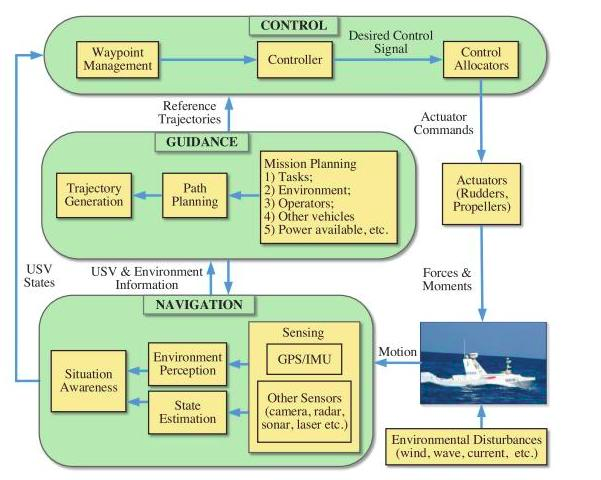
\includegraphics[width=\textwidth]{fig/gnc_system.png}
            \caption{Caption}
            \label{fig:gnc_system}
        \end{figure}
    
        A Figura ~\ref{fig:gnc_system} apresentada por Liu \etal~\cite{LIU201671} mostra o sistema GNC em detalhe apontando suas funções. Tais funções serão brevemente explicadas a seguir.
        
        \begin{enumerate}
            \item \textit{"Navigation":} subsistema responsável pela coleta de informações a respeito do barco (posição, velocidade, etc) e seu entorno (obstáculos estáticos e obstáculos móveis). Essas informações são coletadas por meio de sensores, radares, câmeras, cartas náuticas e mapas. Os dados coletados são enviados para o subsistema \textit{"Guidance"}~\cite{JURAK2020}.
            
            \item \textit{"Guidance":} subsistema responsável por gerenciar os dados da missão atual a ser executada e definir os meios necessários para cumpri-la. Através dos dados obtidos do subsistema \textit{"Navigation"}, as ações necessárias para atingir o objetivo são definidas e enviadas para o subsistema \textit{"Guidance"}~\cite{JURAK2020}.
            
            % As informações referentes ao próprio barco captadas pelo sistema de navegação também vão para o sistema de controle, pois ele precisa saber a posição atual do barco para saber como ele vai atuar para chegar na próxima posição determinada pelo guidance
            \item \textit{"Control":} subsistema que, com base no estado atual do USV obtido pelo subsistema \textit{"Navigation"}, gera os comandos necessários para realizar as ações definidas pelo subsistema \textit{"Guidance"}. Além disso, também é sua responsabilidade executar os comandos gerados diretamente nos atuadores do USV~\cite{JURAK2020}.
        \end{enumerate}
        
        
    
    \section{Regulamentos Internacionais para Prevenção de Colisões no Mar}\label{subchap2:colregs}
        Buscando padronizar as ações tomadas para evitar colisões, a Organização Internacional da Marinha (IMO - do inglês International Marine Organization) definiu uma série de regulamentações para colisão no mar (COLREGS - do inglês COLlision REGulations at Sea)~\cite{JURAK2020}.
        Para que o uso de USV não apresente perigo para outras embarcações, sendo elas triupuladas ou não, é necessário que ele não realize ações inesperadas pelos humanos do barco que se aproxima. Sendo assim, o USV deverá realizar suas ações de acordo com a COLREGS de forma que seja perceptível para o humano que estiver no outro barco~\cite{KUWATA2014110}.
        
        Jurak~\cite{JURAK2020} em seu sistema considerou os encontros \textit{"head-on"}, \textit{"crossing from left"}, \textit{"crossing from right"} e \textit{"overtaking"}. As situações listadas são ilustradas na Figura~\ref{fig:colregs_situations} e serão explicados a seguir: 
        
        \begin{figure}
            \centering
            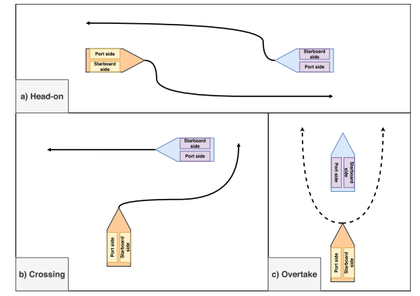
\includegraphics[width=\textwidth]{fig/colregs_situations.png}
            \caption{Caption}
            \label{fig:colregs_situations}
        \end{figure}
        
        \begin{enumerate}
            \item [1] \textit{"head-on":} situação em que as embarcações se encontram frente a frente. Nesse caso, a COLREGS especifíca que ambas as embarcações devem evitar a colisão virando à \textit{"starboard side"} (estibordo) e, por consequência, passando pelo \textit{"port side"} (bombordo) do outro navio.
            
            \item [2] \textit{"crossing from left/right":} situação em que uma embarcação cruzará o caminho da outra. Nesse caso, a embarcação que possuir a outra no seu lado direito (\textit{"startboard side"} - estibordo) é responsável por evitar a colisão contornando a embarcação que se aproxima por trás, realizando uma conversão à direita (\textit{"startboard"} - estibordo). Já a embarcação que possuir a outra no seu lado esquerdo (\textit{"port side"} - bombordo), não deverá mudar seu curso.
            
            \item [3] \textit{"overtaking":} situação em que uma embarcação se encontra em uma velocidade maior do que a embarcação que se encontra à frente. Nesse caso a embarcação que se aproxima pode desviar pelo lado em que não causará uma nova situação de \textit{"overtaking"}.
        \end{enumerate}
        
    
    \section{Prevenção de Colisão}\label{subchap2:prev_col}
        % FALAR AQUI QUE O SUBSISTEMA GUIDANCE É RESPONSÁVEL PELO PROCESSO DE COLLISION AVOIDANCE %
        %subsistema reponsável por analisar os dados recebidos do subsistema \textit{"Navigation"} e encontrar o melhor trajeto possível, através de planejadores, para atingir o objetivo~\cite{JURAK2020}. Portanto, é responsabilidade do subsistema \textit{"Guidance"} executar todas as etapas necessárias para a prevenção de colisão~\cite{HUANG2020451}, que serão abordadas na sessão ~\ref{subchap2:prev_col}.
        
        Prevenção de colisão consiste em um dos principais desafios ao desenvolver um USV~\cite{JURAK2020}. Para que seja possível se mover pelas águas de acordo com as COLREGS, é preciso um meio de identificar as situações de risco.
        
        Huang (2020, p.451) define prevenção de colisão como:
        \begin{directcite}
            \textit{"Prevenção de colisão é o processo em que um navio desvia de sua trajetória planejada para evitar contato físico indesejado em um certo tempo futuro"}
        \end{directcite}
        
        Com isso, Huang\etal~\cite{HUANG2020451} separa o processo de prevenção de colisão nas seguintes etapas: 
        
        \begin{enumerate}
            \item [1] Previsão de Movimento: que prevê estados futuros do OS e dos TSs envolvidos;
            \item [2] Detecção de Conflito: determina se o OS está em risco de colisão;
            \item [3] Resolução de Conflito: encontrará o melhor caminho para evitar a colisão.
        \end{enumerate}
        
        % Trecho explicado de forma mais sucinta pelo enumerate anterior
        %Na Figura~\ref{fig:col_avoid_info_flow} é possível observar o fluxo de informação por entre os módulos que compõe um sistema de evasão de colisão. Em suma, o módulo \textit{"Observer"} coleta informações através de seus sensores e câmeras; \textit{"Motion Prediction"} faz uso dos dados coletados pelo módulo anterior para estimar as futuras posições do OS e do TS; \textit{"Conflict Detection"} ineterpreta as informações fornecidas pelos módulos anteriores para verificar se há o risco de colisão; havendo risco de colisão, o módulo \textit{"Conflict Resolution"} é acionado para determinar as ações necessárias para evadir da situação de risco; o módulo \textit{"Actuator"} executa as ações definidas pelos módulos anteriores~\cite{HUANG2020451}.
        
        As etapas apresentadas podem ser compreendidas como módulos do subsistema \textit{"Guidance"}, que é o responsável por tais ações~\cite{JURAK2020}.
        
        A Figura~\ref{fig:col_avoid_info_flow}, apresentada por Huang\etal~\cite{HUANG2020451}, mostra o fluxo de informação realizada em uma prevenção de colisão. Na imagem, podemos considerar \textit{"Observer"} e \textit{"Actuator"} como módulos dos subsistemas de \textit{"Navigation"} e \textit{"Control"}, respectivamente. Os módulos envoltos pelo pontilhado vermelho compõe o subsistema \textit{"Guidance"}. 
        
        As informações coletadas pelo \textit{"Observer"} são utilizadas pelo módulo \textit{"Motion Prediction"}, quando implementado, para realizar as previsões necessárias. O módulo \textit{"Conflict Detection"} utilizará as informações providas pelo \textit{"Motion Prediction"}, ou \textit{"Observer"}, a fim de identificar se há risco de colisão. Se não houver, as diretivas de caminho e velocidade são enviadas diretamente para o \textit{"Actuator"}. Caso houver risco de colisão, o módulo \textit{"Conflict Resolution"} será acionado para que encontre um caminho seguro para evitar a colisão, consequentemente, gerando diretivas de caminho e velocidade que levarão a um desvio da rota global.
        
        \begin{figure}
            \centering
            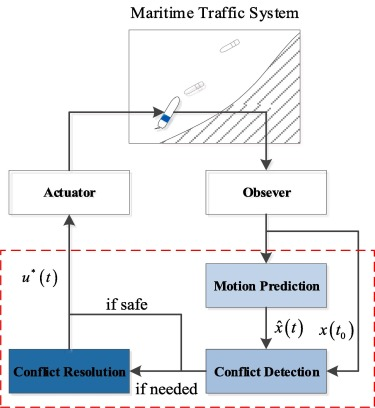
\includegraphics{fig/information_flow.png}
            \caption{Fluxo de informação ~\cite{HUANG2020451}}
            \label{fig:col_avoid_info_flow}
        \end{figure}
        
        